Constraint satisfaction problems(CSP) are mathematical problems defined as a set of objects whose state must satisfy a number of constraints or limitations. One example of a CSP is the game “Sudoku” \\[3ex]

\subsection{Basic terms about CSP:}
\begin{itemize}
\item an assignment is to assign values to some or all variables
\item an assignment that does not violate any constraints is called a consistent assignment. With values from domain D\_i
\item A complete assignment is one in which each variable is assigned
\item a partial assignment is one that assigns value to some of the variables 
\end{itemize}


\textbf{Constraint graph}\\
Binary CSP: each constraint relates at most two variables, e.g: WASA
constraint graph: nodes are variables(e.g. region WA), arcs show constraints(e.g. WASA)\\[3ex]

\textbf{Varieties of Variables}\\
Discrete variables
\begin{itemize}
\item Finite Domains
\item boolean CSPs, include: boolean satisfiability(NP - complete)
\item Sudoku
\item Infinite Domains(Integers, Strings, etc.)

\item job scheduling, variables are start/end days for each job, need a constraint language, e.g. $StartJob_1$ + 5 $\leq  StarJob_3$
\end{itemize}
Continuous variables
\begin{itemize}
\item start /end times for Hubble Telescope observations
\item Unary constraints involve a single variable
\setlength{\itemindent}{3em}
\item $SA \neq Green$
\setlength{\itemindent}{0em}
\item binary constraints involve pairs of variables
\setlength{\itemindent}{3em}
\item $SA \neq WA$
\setlength{\itemindent}{0em}
\item Higher-order constraints involve 3 or more variables	
\setlength{\itemindent}{3em}
\item cryptarithmetic column constraints
\setlength{\itemindent}{0em}
\item Preferences(soft) constraints
\setlength{\itemindent}{3em}
\item red  is better than green
\item CSPs with preference are often with optimization search algorithms constraints optimization problems 
\end{itemize}

\textbf{Node Consistency}\\
If a node is node-consistent if all the value’s domain satisfy the variable’s unary constraints.\\[3ex]

Example:\\
D = {Red, Green, Blue}\\
Variable X\\
X dislikes green, then X starts with D = {Red, Green, Blue}, and becomes node consistent after eliminating {Green}.
X is node consistent with the reduced domain, D={Red, Blue}.\\

\textbf{Arc Consistency}\\
$X_i$ is arc-consistent with respect to another variables $X_j$ if for every value in $X_i$’s current domain $D_i$ there is one value in $X_i$’s domain $D_j$ that satisfies the binary constraint on the arc $(X_i , X_j)$\\[3ex]

Example:\\
Given two variables $X_i$ , $X_j$ with values in {0,1,2,...9} and constraints 
(0,0),(1,1),(2,4),(3,9).\\
To make $X_i$ arc-consistent with respect to $X_j$, we reduce $X_i$’s domain to {0,1,2,3}.\\
To make $X_j$ arc-consistent with respect to $X_i$, we reduce $X_j$’s domain to {0,1,4,9}.\\

\subsection{Arc Consistency Algorithm(AC-3)}
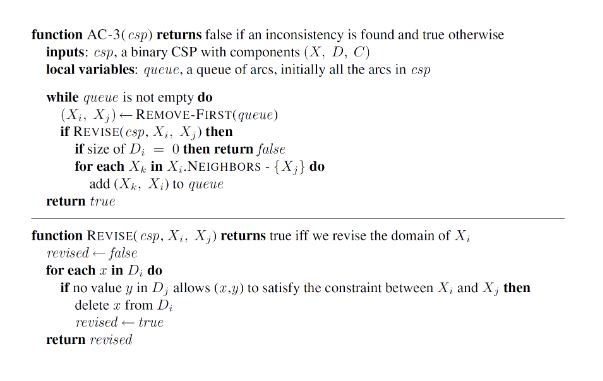
\includegraphics[scale=1]{chap1_pics/1nAyMlelLl-LW-ECO-Akl5AsNAugdRshrNF4o7Q.png} 
\begin{enumerate}
\item initially let a queue contain all arcs
\item remove an arc $(X_i , X_j)$ from the queue and make the variable $X_i$ arc-consistent to $X_j$
\begin{enumerate}
\item IF$ X_i$ domain $D_i$ is unchanged, then check the next arc in the queue
\item IF $X_i$ ‘s domain $D_i$ is revised(smaller), then add all arcs $(X_k, X_i) $in the queue 
\item If $X_i$ ’s domain $D_i$ is empty, then CSP no solution
\end{enumerate}
\item Keep checking all arcs in the queue until the queue is empty 
\end{enumerate}

\subsection{Path consistency}
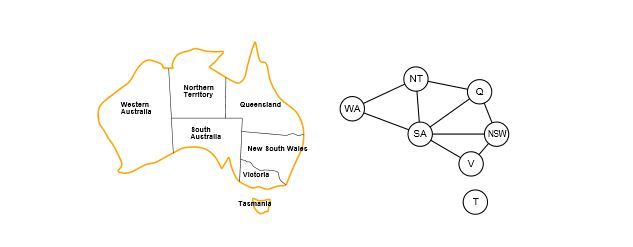
\includegraphics[scale=1]{chap1_pics/patchconsistency.jpeg} 





